\documentclass[12pt]{article}
\usepackage[english]{babel}
\usepackage{natbib}
\usepackage{url}
\usepackage[utf8x]{inputenc}
\usepackage{amsmath}
\usepackage{graphicx}
\graphicspath{{images/}}
\usepackage{parskip}
\usepackage{fancyhdr}
\usepackage{vmargin}
\setmarginsrb{3 cm}{2.5 cm}{3 cm}{2.5 cm}{1 cm}{1.5 cm}{1 cm}{1.5 cm}

\title{UCT Report Template}								% Title
\author{SOW Sokhna Maimouna}								% Author
\date{\today}											% Date

\makeatletter
\let\thetitle\@title
\let\theauthor\@author
\let\thedate\@date

\makeatother

\pagestyle{fancy}
\fancyhf{}
\lhead{\theauthor}
\rhead{\rightmark}
\lfoot{Universite Paris Ouest}
\rfoot{Cosmo Consult}
\cfoot{\thepage}
\renewcommand{\footrulewidth}{0.4pt}%trait horizontal pour le pied de page

\begin{document}

%%%%%%%%%%%%%%%%%%%%%%%%%%%%%%%%%%%%%%%%%%%%%%%%%%%%%%%%%%%%%%%%%%%%%%%%%%%%%%%%%%%%%%%%%

\begin{titlepage}

\includegraphics[scale=0.5]{images/image1.jpg} \hspace*{\stretch{1}}

\includegraphics[scale=0.3]{images/image2.png}
\vspace*{\stretch{4}}

\hrulefill
\begin{center}\bfseries\Huge
     RAPPORT DE STAGE
\end{center}

\begin{center}\bfseries\Huge
	Project Assistant
\end{center}

\begin{center}\bfseries\Huge
Mise en place d'un outil d'agrégation de calendrier et de planification
\end{center}
\hrulefill

\vspace*{4cm}
\textbf{SOW Sokhna Maimouna} \hspace*{\stretch{1}} 
Enseignant Tuteur : \textbf{Marta Rukoz} \\
M1 MIAGE Classique \hspace*{\stretch{1}}
Maître de stage : \textbf{Xavier Garonnat} \\
Année 2016/2017 \\ 
 
\end{titlepage}

%page de garde
\thispagestyle{empty}
\newpage
~

\newpage
\section{Remerciements}
\hspace{1cm} Je tiens tout d’abord à remercier mon tuteur de stage, \textbf{Monsieur Xavier Garonnat}, pour sa disponibilité et son assistance, malgré le peu de temps qu’il a. Il est très attentif et compréhensif. Ses explications et ses conseils à la recherche de solutions meilleures m’ont beaucoup aidée à trouver le chemin adéquate.\\ 

\hspace{1cm} Mes remerciements s’adressent également à mon maître de stage \textbf{Madame Marta Rukoz} pour son attention envers moi et pour sa disponibilité, à mon responsable de formation \textbf{Monsieur Pascal Poizat} pour ses conseils durant toute l’année scolaire et tout le \textbf{corps professionnel} de l’université Paris Nanterre.\\ 

\hspace{1cm} Je remercie également \textbf{Monsieur Jean-Marc Garel} pour sa confiance et toute son aide. Mes remerciements s’adressent également à toute l’équipe de Cosmo Consult particulièrement à \textbf{Monsieur Christophe Reulier} qui m’a bien accueillie à bras ouvert et m’a beaucoup aidé à m’intégrer dans l’entreprise.\\

\hspace{1cm} Et enfin je dis un grand merci à \textbf{ma grande sœur} qui m’a toujours soutenue et aidée dans mes études, à mes parents et à tous mes proches.


%%%%%%%%%%%%%%%%%%%%%%%%%%%%%%%%%%%%%%%%%%%%%%%%%%%%%%%%%%%%%%%%%%%%%%%%%%%%%%%%%%%%%%%%%
\newpage
\tableofcontents
\pagebreak

%%%%%%%%%%%%%%%%%%%%%%%%%%%%%%%%%%%%%%%%%%%%%%%%%%%%%%%%%%%%%%%%%%%%%%%%%%%%%%%%%%%%%%%%%

\section{Introduction}
\hspace{1cm} Dans le cadre de l'obtention du diplôme de M1 MIAGE, nous sommes appelés à effectuer un stage obligatoire de 3 mois minimum. Ce stage nous permettra de mettre en pratique les enseignements théoriques de la formation à savoir la gestion de projet et/ou le développement informatique et de nous familialiser au monde professionnel.\\
 
\hspace{1cm} J'ai eu la chance d'être accueillie comme stagiaire chez Cosmo Consult, du 03 avril au 14 août 2017. Ayant déjà fait un stage en tant que développeur, j'ai saisi l'opportunité d'être dans une formation à double compétence pour me lancer, cette année dans ce stage comme assistante de projet.\\ 
 
\hspace{1cm} Dans un premier temps je vous présenterai l'entreprise, son historique, sa structuration et ses activités. Ensuite j'aborderai le déroulement de mon stage, mes principales missions au sein de Cosmo Consult France avec les méthodes adoptées pour mener à bout ce qui m'a été confiée et les problèmes rencontrés. Et pour finir je ferais un bilan pour exprimer ce que ce stage m'a apportée.

\newpage
\section{Cosmo Consult}
	\subsection{Présentation du groupe}
\hspace{1cm} Cosmo Consult International a été créé en 1996. C'est une société européenne indépendante, présente en Allemagne, Espagne, Suède et France, et qui est devenue l'un des leaders européens de l’intégration des solutions Microsoft Dynamics et éditeur de logiciels métiers basés sur les technologies Microsoft.  Cosmo accompagne ses clients, PME/PMI et filiales de grands groupes dans leurs projets de transformation numérique et d’évolution de leur Système d’Information.\\

\hspace{1cm} De nos jours elle compte près de 650 collaborateurs répartis sur 20 succursales en Europe et plus de 2000 clients dans le monde entier. Elle est dans le top 3 de l'intégration Dynamics en Europe et dans le top 5 des partenaires Dynamics dans le monde. Elle a une performance durable et soutenue avec un chiffre d'affaire de près de 19 millions d'euros en 2012 et 90 millions d'euros en 2016. 

	\subsection{Présentation de Cosmo Consult France}
\hspace{1cm} La France rejoint le groupe en juin 2015. Cosmo Consult France est une filiale en pleine expansion avec un plan de développement ambitieux sur les 3 prochaines années. Elle est partenaire stratégique Microsoft avec une équipe Dynamics NAV expérimentée dans :
\begin{itemize}
	\item L’intégration :
		\begin{itemize}
			\item L’implémentation ERP
			\item Business Intelligence
			\item Content Management
		\end{itemize}
		
	\item L’évolution du SI :
		\begin{itemize}
			\item Optimisation
			\item Migration
		\end{itemize}	 
	\item Le support  
	\item L'éditeur de solution métiers
\end{itemize}

\hspace{1cm} Cosmo Consult est devenue l'un des plus grands fournisseurs de logiciels sectoriels et de gestion pour les PME et les grandes entreprises, basés sur les dernières technologies Microsoft et QlikView.\\

	\subsection{L'organisation de Cosmo Consult}
\hspace{1cm}L'équipe Cosmo Consult France est composée d'une direction des opérations et d'une direction commerciale. Au sein de ces deux directions, nous retrouvons des chefs de projets, des responsables marketing, des développeurs, des chefs d'équipe de soutien, des hauts comptables des consultants fonctionnels et des consultants séniors.\\

Ci-dessous l'organigramme de toute l'équipe Cosmo Consult France.
\begin{center}
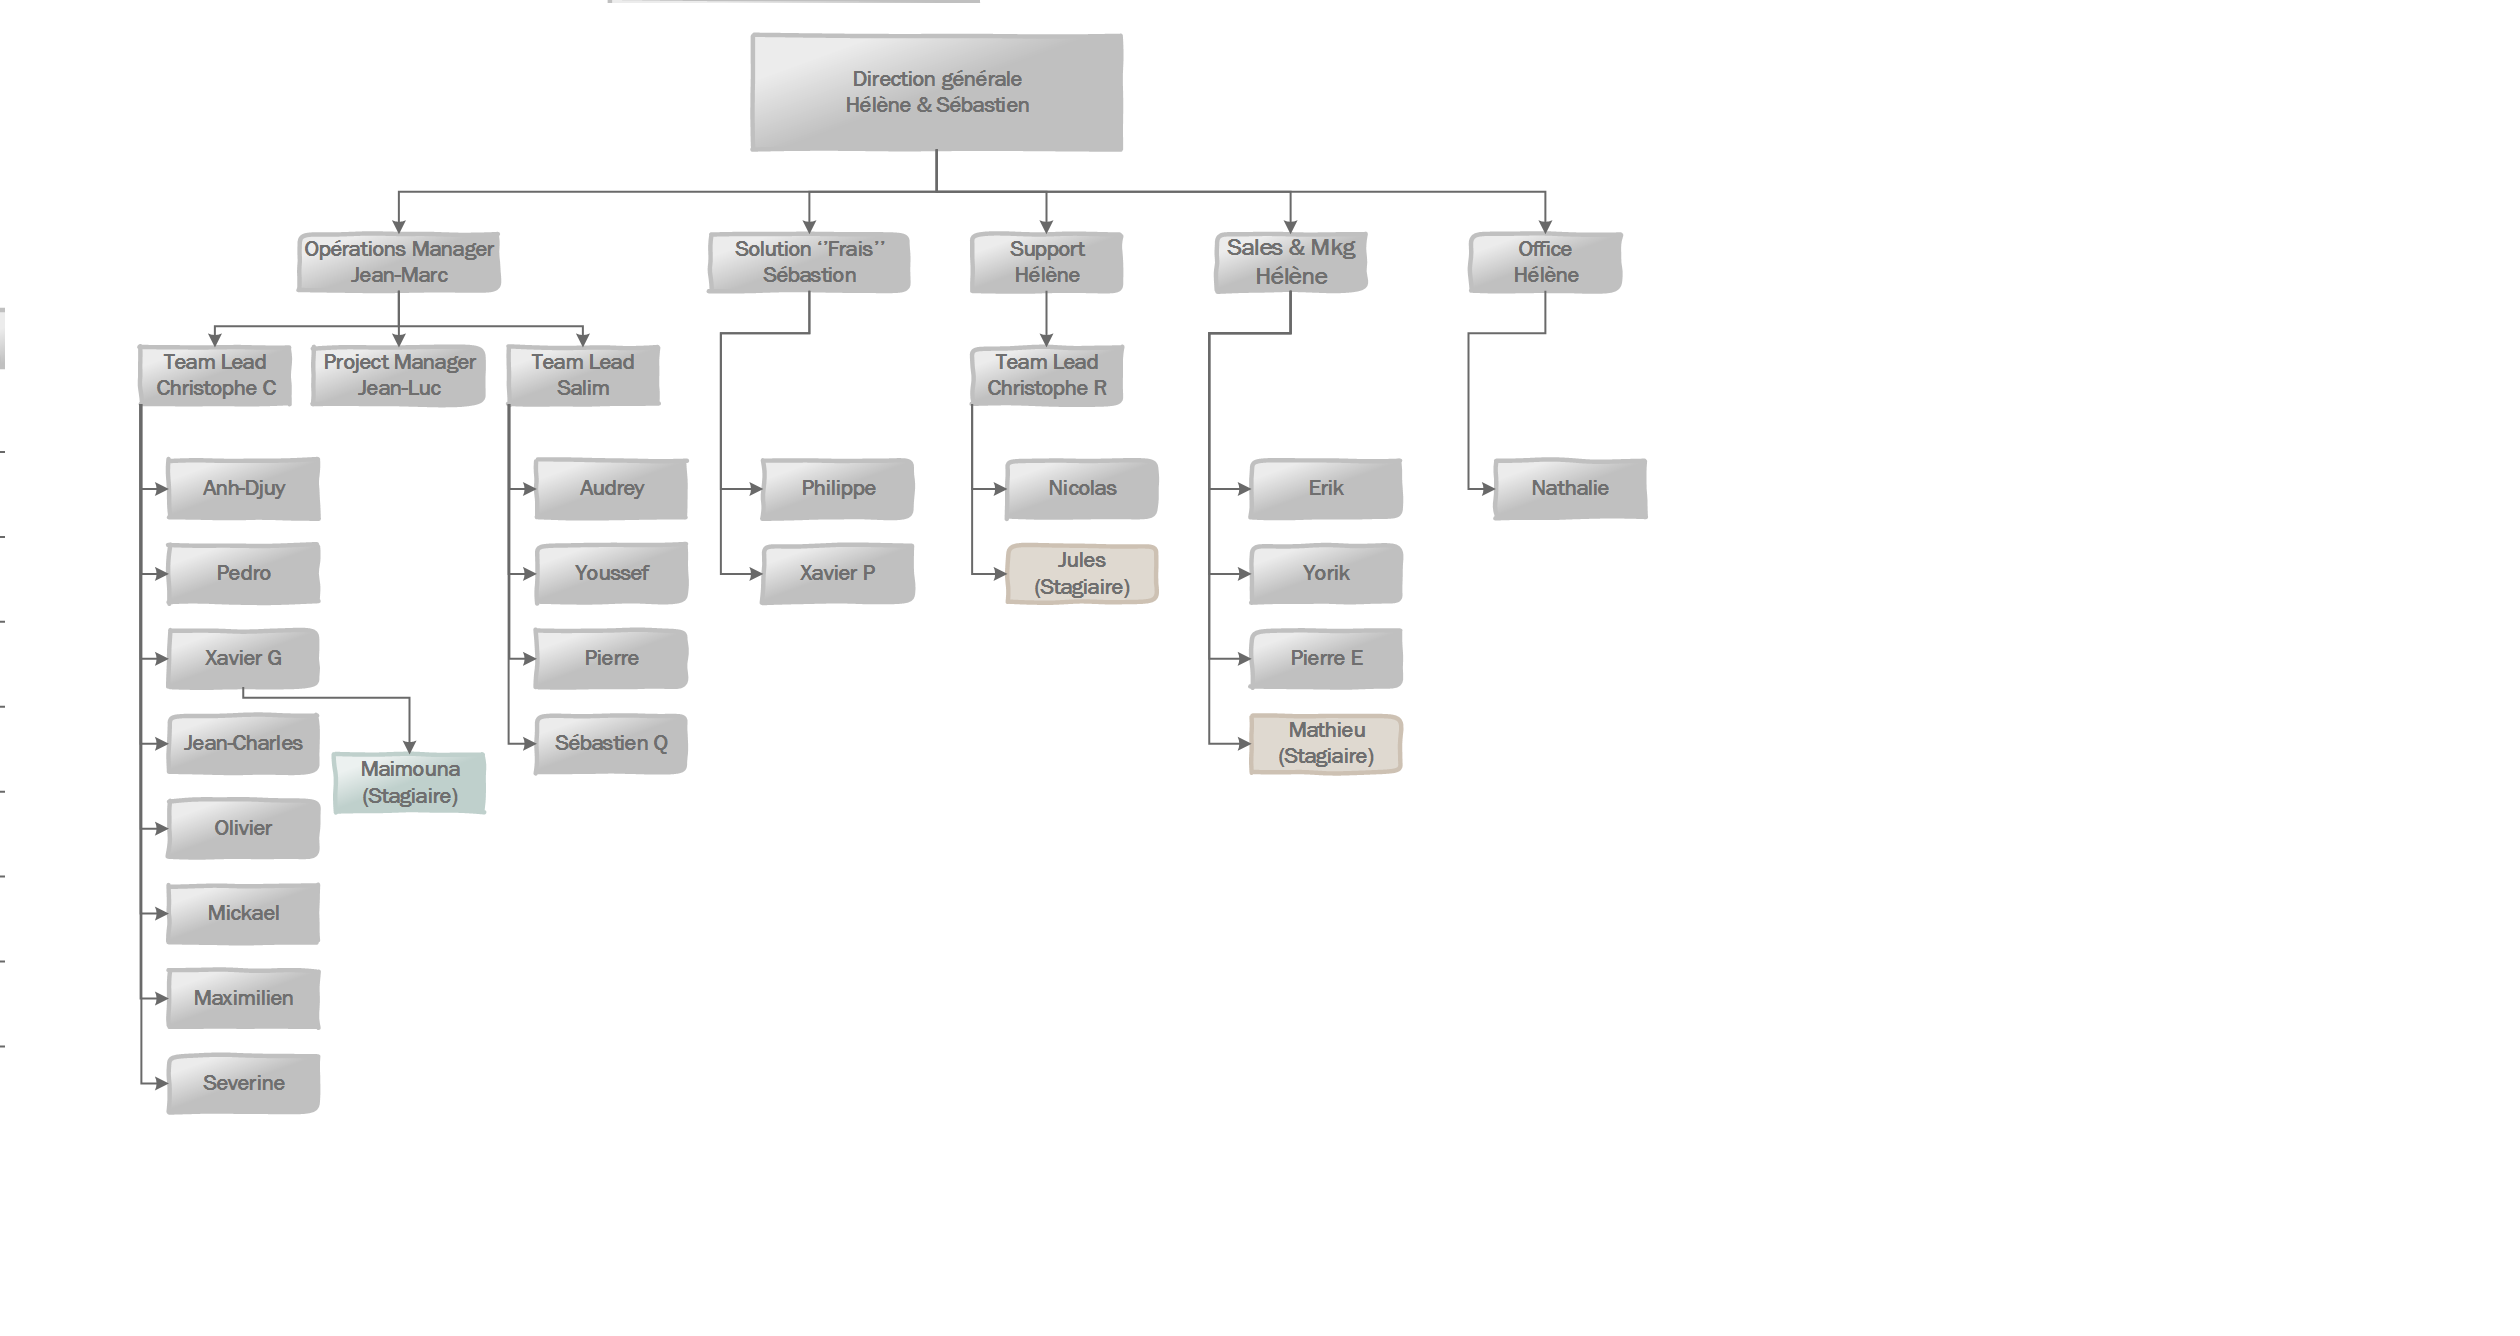
\includegraphics[scale=0.5]{images/figure1.png}
\vspace*{\stretch{-10}}
\underline{\textbf{Figure 1 : Organigramme de Cosmo}}
\end{center}

	\subsection{Les activités de Cosmo Consult France}
\hspace{1cm} Cosmo Consult France est devenu le leader en France sur le marché des solutions Dynamics et des services de conseil et d'intégration auprès de sociétés nationales et internationales. Cosmo Consult France offre les solutions : 
\begin{itemize}
	\item\textbf{ ERP Gestion à l'affaire} : pour les équipements industriels, producteurs d'équipements spéciaux, les sociétés de services, de conseil et d'ingénierie, les bureaux d'études…
	
	\item \textbf{ERP Discrete Manufacturing} : pour la fabrication d'équipements spécifiques ou configurables, en petite séries ou à la commande, le service après-vente, les modes de gestion engineer-to-order, make-to-order…
	
	\item \textbf{ERP Process Manufacturing} : pour les secteurs de la plasturgie, de la chimie fine, de l'industrie du verre et de la céramique, des colles, vernis, peintures…
	
	\item \textbf{ERP Life Sciences} : pour les secteurs de la pharmacie, des biotechnologies, des compléments alimentaires, de la cosmétique et les fabricants d'équipements médicaux…
	
\end{itemize}
\section{Déroulement du stage}
	\subsection{Planning}
	\subsection{Objectif du stage}
	
\section{Missions}
	\subsection{Description de la mission}
	\subsection{Méthodes de travail}
		\subsubsection{Réunions avec les allemands}
		\subsubsection{Réunions avec les espagnols}
	\subsection{Démarches de la résolution}
		\subsubsection{Collecte des besoins}
		\subsubsection{Définition du périmètre}
		\subsubsection{Etude de marché}	
		\subsubsection{Choix final}
		
\section{Bilan}
\section{Bibliographie}
\section{Annexes}
\section{Glossaire}

ogjiugyfrdipolkjhgfds

%\newpage
%\bibliographystyle{plain}
%\bibliography{biblist}

\end{document}
